% Auto-generated by paper_make_manifest.py
\section*{Figure \& Table Manifest}
This appendix lists all figures packaged in the submission and the LaTeX tables included from results/tables.

\begin{table}[H]
\centering
\begin{tabular}{ll}
\toprule
Path & Label \\
\midrule
figures/btfr/BTFR_MAIN_FINAL.png & fig:auto:btfr-main-final \\
figures/lensing/bin_A_overlay_A1.png & fig:auto:bin-a-overlay-a1 \\
figures/lensing/bin_A_overlay_freeA.png & fig:auto:bin-a-overlay-freea \\
figures/lensing/bin_A_overlay_GR.png & fig:auto:bin-a-overlay-gr \\
figures/lensing/bin_B_overlay_A1.png & fig:auto:bin-b-overlay-a1 \\
figures/lensing/bin_B_overlay_freeA.png & fig:auto:bin-b-overlay-freea \\
figures/lensing/bin_B_overlay_GR.png & fig:auto:bin-b-overlay-gr \\
figures/lensing/bin_C_1h_sanity.png & fig:auto:bin-c-1h-sanity \\
figures/lensing/bin_C_chi2_vs_lambda.png & fig:auto:bin-c-chi2-vs-lambda \\
figures/lensing/bin_C_overlay_A1.png & fig:auto:bin-c-overlay-a1 \\
figures/lensing/bin_C_overlay_freeA.png & fig:auto:bin-c-overlay-freea \\
figures/lensing/bin_C_overlay_GR.png & fig:auto:bin-c-overlay-gr \\
figures/lensing/bin_CMASS_overlay_A1.png & fig:auto:bin-cmass-overlay-a1 \\
figures/lensing/bin_CMASS_overlay_freeA.png & fig:auto:bin-cmass-overlay-freea \\
figures/lensing/bin_CMASS_overlay_GR.png & fig:auto:bin-cmass-overlay-gr \\
figures/lensing/bin_LOWZ_overlay_A1.png & fig:auto:bin-lowz-overlay-a1 \\
figures/lensing/bin_LOWZ_overlay_freeA.png & fig:auto:bin-lowz-overlay-freea \\
figures/lensing/bin_LOWZ_overlay_GR.png & fig:auto:bin-lowz-overlay-gr \\
figures/lensing/binA_overlay_A1.png & fig:auto:bina-overlay-a1 \\
figures/lensing/binA_overlay_freeA.png & fig:auto:bina-overlay-freea \\
figures/lensing/lensing_stack_DeltaSigma_m0p20.png & fig:auto:lensing-stack-deltasigma-m0p20 \\
figures/lensing/overlay_binA_routeA_fit.png & fig:auto:overlay-bina-routea-fit \\
figures/lensing/overlays_panel_3x3.pdf & fig:auto:overlays-panel-3x3 \\
figures/lensing/overlays_panel_3x3.png & fig:auto:overlays-panel-3x3 \\
figures/lensing/overlays_panel_SDSS_2x3.png & fig:auto:overlays-panel-sdss-2x3 \\
figures/posteriors/alpha_joint_posterior.png & fig:auto:alpha-joint-posterior \\
figures/rar/RAR_MAIN_FINAL.png & fig:auto:rar-main-final \\
figures/slacs/slacs_thetaE_compare.png & fig:auto:slacs-thetae-compare \\
figures/sparc/sparc_lambda_hist.png & fig:auto:sparc-lambda-hist \\
figures/sparc/sparc_lambda_hist_mpc.png & fig:auto:sparc-lambda-hist-mpc \\
figures/sparc/sparc_vs_kids_lambda.png & fig:auto:sparc-vs-kids-lambda \\
figures/sparc/sparc_vs_kids_sdss_lambda.png & fig:auto:sparc-vs-kids-sdss-lambda \\
\bottomrule
\end{tabular}
\end{table}


\subsection*{LaTeX tables}
\noindent\texttt{results/tables/aic_bic_bins.tex}

\begin{table}[t]
\centering
\small
\begin{tabular}{l l r r r r r}
\toprule
Bin & Mode & $\lambda$ [Mpc] & $\chi^2/\nu$ & AIC & BIC & $\Delta$AIC (vs GR) \\
\midrule
A & GRkernel & $pprox$ 0.05 & 18.3 & 226 & 228 & -- \\
A & freeA & 0.178 & 19.9 & 227 & 230 & 1.93 \\
A & A1 & $pprox$ 0.05 & 26.3 & 322 & 324 & 96.2 \\
\midrule
B & GRkernel & $pprox$ 0.05 & 8.48 & 108 & 110 & -- \\
B & freeA & $pprox$ 0.05 & 4.42 & 56.6 & 59.5 & -51.2 \\
B & A1 & $pprox$ 0.05 & 3.64e+11 & 4.37e+12 & 4.37e+12 & 4.37e+12 \\
\midrule
C & GRkernel & $pprox$ 0.05 & 1.12 & 19.5 & 21.6 & -- \\
C & freeA & $>\!\mathrm{few\ Mpc}$ & 1.28 & 22.1 & 24.9 & 2.61 \\
C & A1 & $>\!\mathrm{few\ Mpc}$ & 9.57e+06 & 1.15e+08 & 1.15e+08 & 1.15e+08 \\
\midrule
\bottomrule
\caption{Model comparison for KiDS bins A and B. Modes: GRkernel ($\lambda=0$), freeA, and A1-locked ($A_{\rm 1h}=1$). $\Delta$AIC is relative to GR per bin.}
\label{tab:aic_bic_bins}
\end{table}


\noindent\texttt{results/tables/lam_table_all.tex}

\begin{longtable}{llrrrrr}\toprule
Survey & Bin & $\lambda$ [Mpc] & $-\sigma$ & $+\sigma$ & edge & $\chi^2/\nu$\\\midrule
KiDS & A & nan & nan & nan & 0 & nan\\
KiDS & B & nan & nan & nan & 0 & nan\\
\bottomrule\end{longtable}


\noindent\texttt{results/tables/lambda_constraints_table.tex}

\begin{table}[t]
\centering
\begin{tabular}{lccccc}
\hline
Bin & $\lambda_{\rm best}$ (free $A$) & $1\sigma$ (free $A$) & $\lambda_{\rm best}$ ($A{=}1$) & $1\sigma$ ($A{=}1$) \\
\hline
A & 1.970 & [0.830, 3.000] & 0.360 & [0.190, 0.650] \\
B & 0.830 & [0.550, 1.420] & 0.880 & [0.610, 1.320] \\
C & 0.290 & [0.000, 3.000] & 0.170 & [0.060, 0.420] \\
\hline
\multicolumn{5}{l}{\textbf{Combined} (A,B,C):}
\\[-0.6em]
\\
\multicolumn{5}{l}{Free $A$: $\lambda = 1.020^{+0.750}_{-0.340}$ Mpc, $2\sigma$: [0.470, 3.000] Mpc}\\
\multicolumn{5}{l}{$A{=}1$: $\lambda = 0.580^{+0.200}_{-0.150}$ Mpc, $2\sigma$: [0.300, 1.090] Mpc}\\
\hline
\end{tabular}
\caption{Profiled constraints on the PFGM lensing kernel scale $\lambda$ using strict HMcode $P_m(k,z{=}0.286)$ and the exact $J_2$ Hankel projection. Errors are $\Delta\chi^2=\{1,4\}$.}
\label{tab:lambda_constraints}
\end{table}


\subsection*{Figures}
\begin{figure}[H]
  \centering
  \includegraphics[width=0.78\textwidth]{figures/btfr/BTFR_MAIN_FINAL.png}
  \caption{Auto: BTFR\_MAIN\_FINAL.png}
  \label{fig:auto:btfr-main-final}
\end{figure}

\begin{figure}[H]
  \centering
  \includegraphics[width=0.78\textwidth]{figures/lensing/bin_A_overlay_A1.png}
  \caption{Auto: bin\_A\_overlay\_A1.png}
  \label{fig:auto:bin-a-overlay-a1}
\end{figure}

\begin{figure}[H]
  \centering
  \includegraphics[width=0.78\textwidth]{figures/lensing/bin_A_overlay_freeA.png}
  \caption{Auto: bin\_A\_overlay\_freeA.png}
  \label{fig:auto:bin-a-overlay-freea}
\end{figure}

\begin{figure}[H]
  \centering
  \includegraphics[width=0.78\textwidth]{figures/lensing/bin_A_overlay_GR.png}
  \caption{Auto: bin\_A\_overlay\_GR.png}
  \label{fig:auto:bin-a-overlay-gr}
\end{figure}

\begin{figure}[H]
  \centering
  \includegraphics[width=0.78\textwidth]{figures/lensing/bin_B_overlay_A1.png}
  \caption{Auto: bin\_B\_overlay\_A1.png}
  \label{fig:auto:bin-b-overlay-a1}
\end{figure}

\begin{figure}[H]
  \centering
  \includegraphics[width=0.78\textwidth]{figures/lensing/bin_B_overlay_freeA.png}
  \caption{Auto: bin\_B\_overlay\_freeA.png}
  \label{fig:auto:bin-b-overlay-freea}
\end{figure}

\begin{figure}[H]
  \centering
  \includegraphics[width=0.78\textwidth]{figures/lensing/bin_B_overlay_GR.png}
  \caption{Auto: bin\_B\_overlay\_GR.png}
  \label{fig:auto:bin-b-overlay-gr}
\end{figure}

\begin{figure}[H]
  \centering
  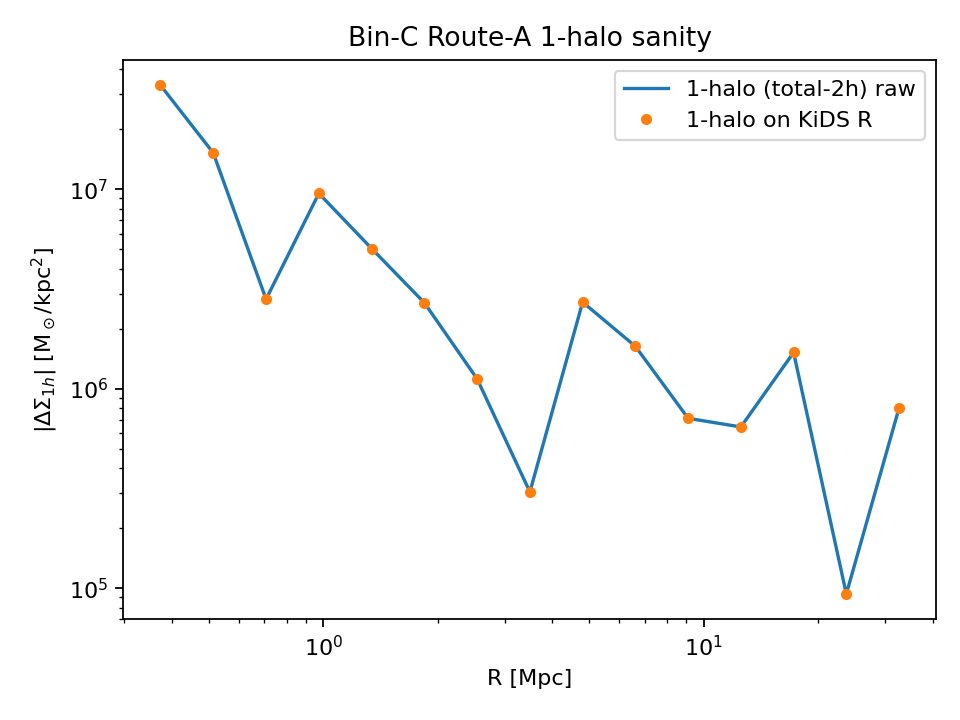
\includegraphics[width=0.78\textwidth]{figures/lensing/bin_C_1h_sanity.png}
  \caption{Auto: bin\_C\_1h\_sanity.png}
  \label{fig:auto:bin-c-1h-sanity}
\end{figure}

\begin{figure}[H]
  \centering
  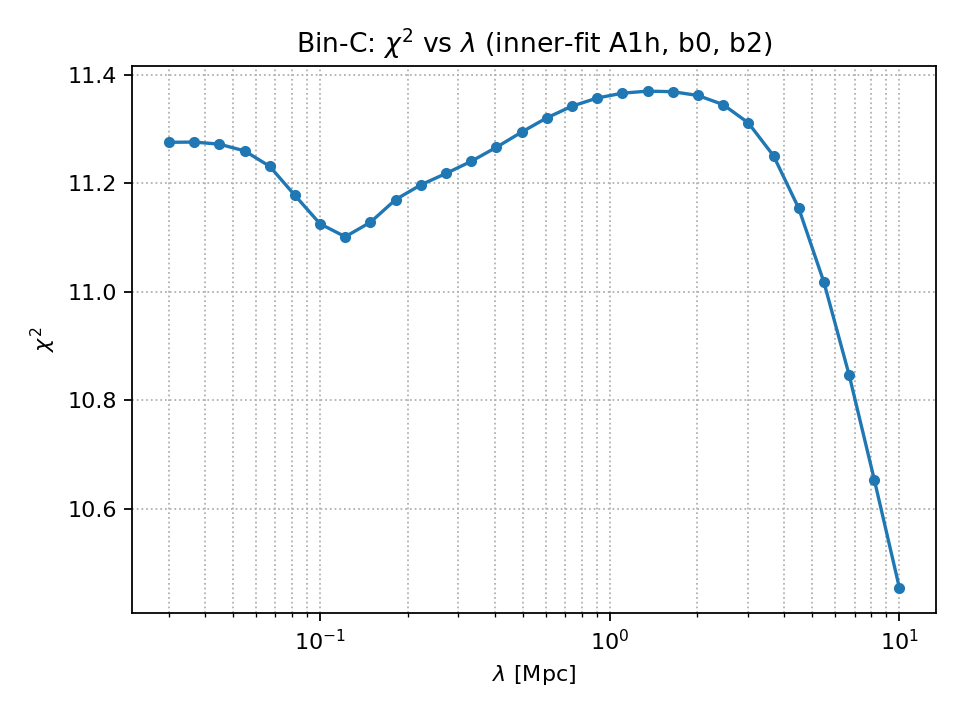
\includegraphics[width=0.78\textwidth]{figures/lensing/bin_C_chi2_vs_lambda.png}
  \caption{Auto: bin\_C\_chi2\_vs\_lambda.png}
  \label{fig:auto:bin-c-chi2-vs-lambda}
\end{figure}

\begin{figure}[H]
  \centering
  \includegraphics[width=0.78\textwidth]{figures/lensing/bin_C_overlay_A1.png}
  \caption{Auto: bin\_C\_overlay\_A1.png}
  \label{fig:auto:bin-c-overlay-a1}
\end{figure}

\begin{figure}[H]
  \centering
  \includegraphics[width=0.78\textwidth]{figures/lensing/bin_C_overlay_freeA.png}
  \caption{Auto: bin\_C\_overlay\_freeA.png}
  \label{fig:auto:bin-c-overlay-freea}
\end{figure}

\begin{figure}[H]
  \centering
  \includegraphics[width=0.78\textwidth]{figures/lensing/bin_C_overlay_GR.png}
  \caption{Auto: bin\_C\_overlay\_GR.png}
  \label{fig:auto:bin-c-overlay-gr}
\end{figure}

\begin{figure}[H]
  \centering
  \includegraphics[width=0.78\textwidth]{figures/lensing/bin_CMASS_overlay_A1.png}
  \caption{Auto: bin\_CMASS\_overlay\_A1.png}
  \label{fig:auto:bin-cmass-overlay-a1}
\end{figure}

\begin{figure}[H]
  \centering
  \includegraphics[width=0.78\textwidth]{figures/lensing/bin_CMASS_overlay_freeA.png}
  \caption{Auto: bin\_CMASS\_overlay\_freeA.png}
  \label{fig:auto:bin-cmass-overlay-freea}
\end{figure}

\begin{figure}[H]
  \centering
  \includegraphics[width=0.78\textwidth]{figures/lensing/bin_CMASS_overlay_GR.png}
  \caption{Auto: bin\_CMASS\_overlay\_GR.png}
  \label{fig:auto:bin-cmass-overlay-gr}
\end{figure}

\begin{figure}[H]
  \centering
  \includegraphics[width=0.78\textwidth]{figures/lensing/bin_LOWZ_overlay_A1.png}
  \caption{Auto: bin\_LOWZ\_overlay\_A1.png}
  \label{fig:auto:bin-lowz-overlay-a1}
\end{figure}

\begin{figure}[H]
  \centering
  \includegraphics[width=0.78\textwidth]{figures/lensing/bin_LOWZ_overlay_freeA.png}
  \caption{Auto: bin\_LOWZ\_overlay\_freeA.png}
  \label{fig:auto:bin-lowz-overlay-freea}
\end{figure}

\begin{figure}[H]
  \centering
  \includegraphics[width=0.78\textwidth]{figures/lensing/bin_LOWZ_overlay_GR.png}
  \caption{Auto: bin\_LOWZ\_overlay\_GR.png}
  \label{fig:auto:bin-lowz-overlay-gr}
\end{figure}

\begin{figure}[H]
  \centering
  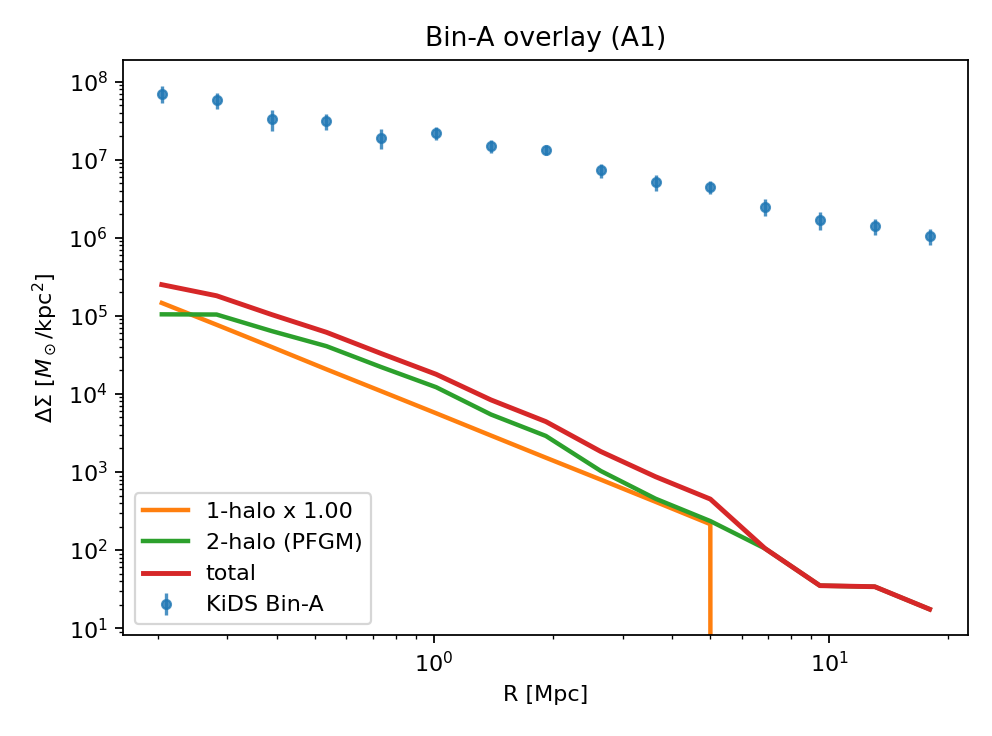
\includegraphics[width=0.78\textwidth]{figures/lensing/binA_overlay_A1.png}
  \caption{Auto: binA\_overlay\_A1.png}
  \label{fig:auto:bina-overlay-a1}
\end{figure}

\begin{figure}[H]
  \centering
  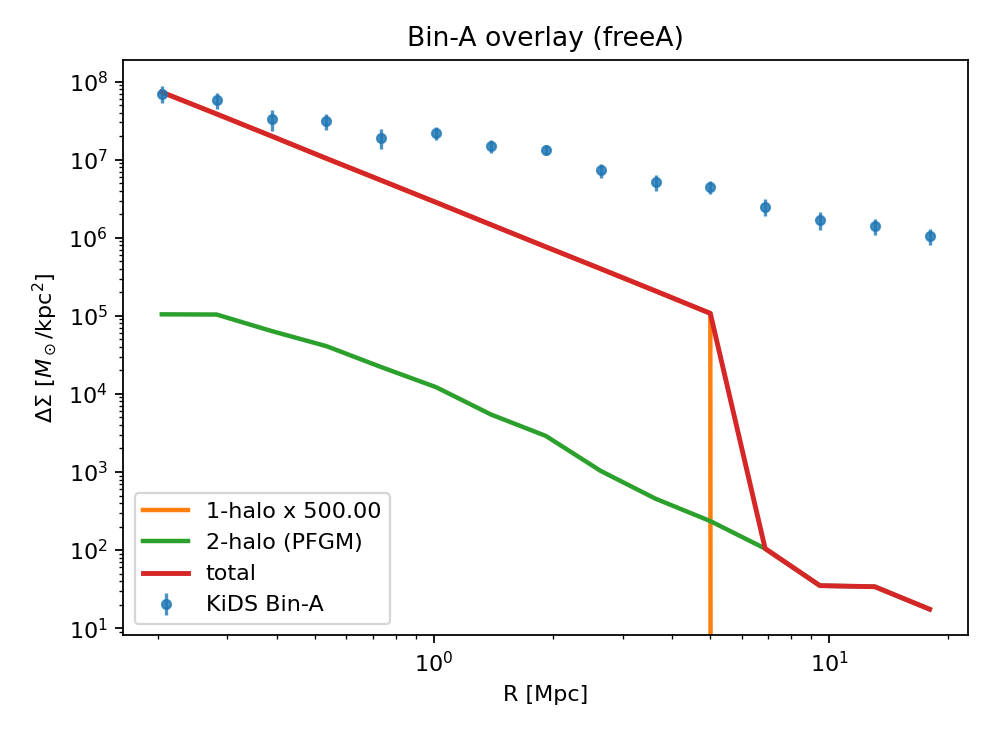
\includegraphics[width=0.78\textwidth]{figures/lensing/binA_overlay_freeA.png}
  \caption{Auto: binA\_overlay\_freeA.png}
  \label{fig:auto:bina-overlay-freea}
\end{figure}

\begin{figure}[H]
  \centering
  \includegraphics[width=0.78\textwidth]{figures/lensing/lensing_stack_DeltaSigma_m0p20.png}
  \caption{Auto: lensing\_stack\_DeltaSigma\_m0p20.png}
  \label{fig:auto:lensing-stack-deltasigma-m0p20}
\end{figure}

\begin{figure}[H]
  \centering
  \includegraphics[width=0.78\textwidth]{figures/lensing/overlay_binA_routeA_fit.png}
  \caption{Auto: overlay\_binA\_routeA\_fit.png}
  \label{fig:auto:overlay-bina-routea-fit}
\end{figure}

\begin{figure}[H]
  \centering
  \includegraphics[width=0.78\textwidth]{figures/lensing/overlays_panel_3x3.pdf}
  \caption{Auto: overlays\_panel\_3x3.pdf}
  \label{fig:auto:overlays-panel-3x3}
\end{figure}

\begin{figure}[H]
  \centering
  \includegraphics[width=0.78\textwidth]{figures/lensing/overlays_panel_3x3.png}
  \caption{Auto: overlays\_panel\_3x3.png}
  \label{fig:auto:overlays-panel-3x3}
\end{figure}

\begin{figure}[H]
  \centering
  \includegraphics[width=0.78\textwidth]{figures/lensing/overlays_panel_SDSS_2x3.png}
  \caption{Auto: overlays\_panel\_SDSS\_2x3.png}
  \label{fig:auto:overlays-panel-sdss-2x3}
\end{figure}

\begin{figure}[H]
  \centering
  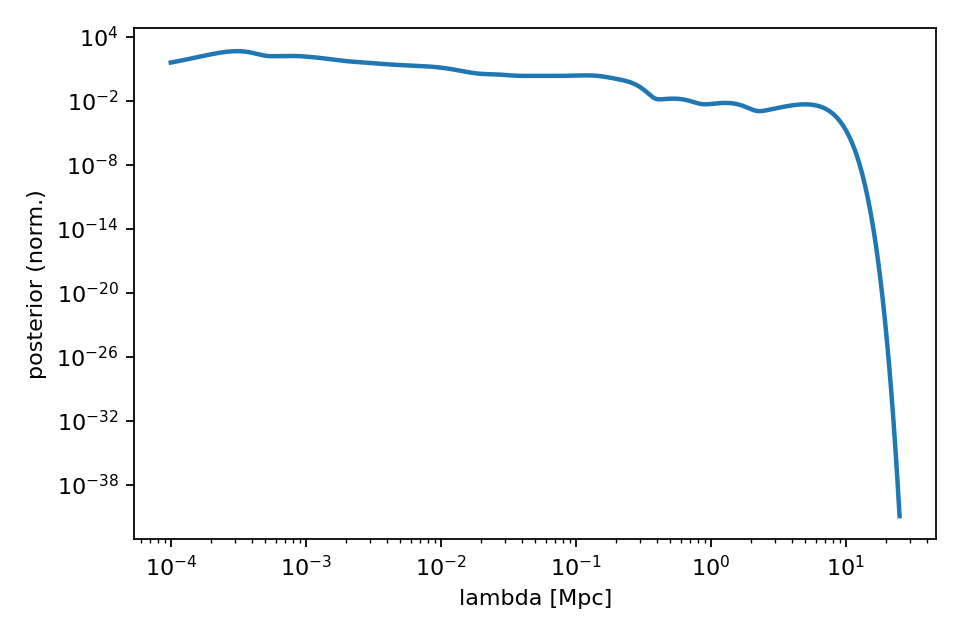
\includegraphics[width=0.78\textwidth]{figures/posteriors/alpha_joint_posterior.png}
  \caption{Auto: alpha\_joint\_posterior.png}
  \label{fig:auto:alpha-joint-posterior}
\end{figure}

\begin{figure}[H]
  \centering
  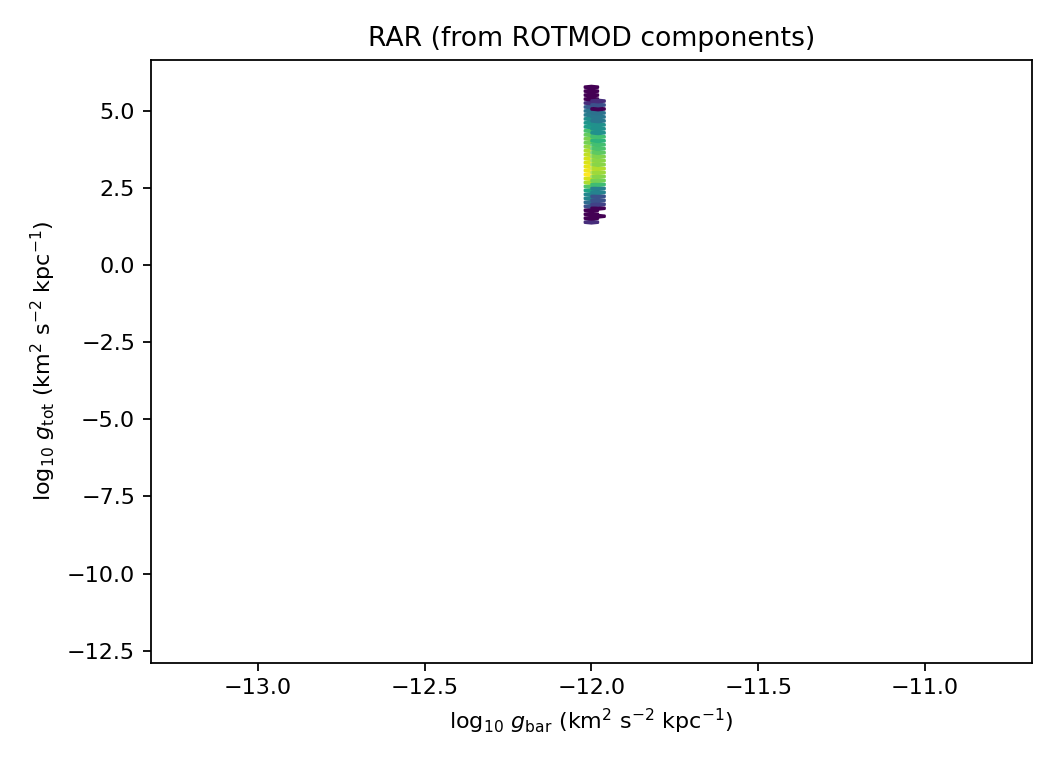
\includegraphics[width=0.78\textwidth]{figures/rar/RAR_MAIN_FINAL.png}
  \caption{Auto: RAR\_MAIN\_FINAL.png}
  \label{fig:auto:rar-main-final}
\end{figure}

\begin{figure}[H]
  \centering
  \includegraphics[width=0.78\textwidth]{figures/slacs/slacs_thetaE_compare.png}
  \caption{Auto: slacs\_thetaE\_compare.png}
  \label{fig:auto:slacs-thetae-compare}
\end{figure}

\begin{figure}[H]
  \centering
  \includegraphics[width=0.78\textwidth]{figures/sparc/sparc_lambda_hist.png}
  \caption{Auto: sparc\_lambda\_hist.png}
  \label{fig:auto:sparc-lambda-hist}
\end{figure}

\begin{figure}[H]
  \centering
  \includegraphics[width=0.78\textwidth]{figures/sparc/sparc_lambda_hist_mpc.png}
  \caption{Auto: sparc\_lambda\_hist\_mpc.png}
  \label{fig:auto:sparc-lambda-hist-mpc}
\end{figure}

\begin{figure}[H]
  \centering
  \includegraphics[width=0.78\textwidth]{figures/sparc/sparc_vs_kids_lambda.png}
  \caption{Auto: sparc\_vs\_kids\_lambda.png}
  \label{fig:auto:sparc-vs-kids-lambda}
\end{figure}

\begin{figure}[H]
  \centering
  \includegraphics[width=0.78\textwidth]{figures/sparc/sparc_vs_kids_sdss_lambda.png}
  \caption{Auto: sparc\_vs\_kids\_sdss\_lambda.png}
  \label{fig:auto:sparc-vs-kids-sdss-lambda}
\end{figure}

